\chapter{Circuit Results Discussion and Summary}
This chapter presents the results of our read-out circuit and the summary of this thesis.
The layout of the circuit is given in \ref{fig:layout}

\begin{figure}[!htbp]
    \centering
    % \includegraphics[width=0.4\textwidth] {images/chapter5/DCMode.png}
    \caption{}
    \label{fig:layout}
\end{figure}

\section{Fronted Circuit and DC-sweep mode}
\begin{figure}[tbh!p]
    \centering
        \includegraphics[width=0.5\textwidth] {images/chapter5/DCMode.PNG}
    \caption{The fronted circuit}
    \label{fig:frontedCIrcuit}
\end{figure}
As in Fig.\ref{fig:frontedCIrcuit}(a), the fronted circuit includes a biasing current source (Ibias), transimpedance amplifier (TIA) and an operational amplifier (OP).
These three circuit blocks combined with the nanowire device (SiNW) form a feedback structure, which is the DC-sweep mode of our circuit.

\subsection{Ibias}
\begin{figure}[tbh!p]
    \centering
        \includegraphics[width=0.3\textwidth] {images/chapter5/mirror.PNG}
    \caption{The fronted circuit}
    \label{fig:mirror_ch6}
\end{figure}
The Fig.\ref{fig:mirror_ch6} is the schematic of the Ibias.
By changing the resistance of the external Res and measuring the current, we obtained the result shown in Fig.\ref{fig:chip:mirror}.

\subsection{Ibias}

\subsection{TIA}
The Fig.\ref{fig:chip:TIA} shows



\subsection{OP} \label{sec:ch6:OP}
By applying a sinusoidal signal to the negative input of OP, we found that the gain of OP is about $2k$ (Fig.\ref{fig:chip:OPGain}).
However, the gain of OP was designed to be more than $5k$.

We will discuss this problem in the following section.
\begin{figure}[tbh!p]
    \centering
        \includegraphics[width=0.8\textwidth] {images/chapter6/Problem_OPGain.png}
    \caption{The output voltage of the OP when the negative input is applied with a sinusoidal signal. This input sinusoidal signal has frequency of $1$Hz and amplitude of $1m V$.
            The positive input of OP is biased with a constant voltage generated by the chip.
            The output signal has amplitude around $2 V$, which means that the gain of OP is about $2k$.}
    \label{fig:chip:OPGain}
\end{figure}

\subsection{Measurement with the DC-sweep Mode Circuit and the Low-current Defect Problem}
\begin{figure}[tbh!p]
    \centering
        \includegraphics[width=0.5\textwidth] {images/chapter6/DCMode.png}
    \caption{DC-sweep mode circuit}
    \label{fig:chip:DCmode}
\end{figure}

With the the DC-sweep mode circuit (Fig.\ref{fig:chip:DCmode}), we swept Ibias and measured $V_G$ and $I_D$ to obtain the $I_D$-$V_G$ and $I_{bias}$-$V_G$ curves (Fig.\ref{fig:chip:IdIbiasVG}).
The chip works well when $I_bias$ is larger than $1\mu A$.
The overlap between two curves implies that $I_D$ follows Ibias and $V_G$ consequently alters due to the feedback mechanism.

When current becomes low, the circuit fails to prompt nanowire follows the biasing current.
This phenomenon could be reasonable because the $g_m$ becomes low and the feedback ability of the circuit may be not strong enough to push the gate of nanowire.
However, when design the circuit (chapter 5), we expected this happens for $g_m$ below $200n$.
The Fig.\ref{fig:chip:gmId} indicates the circuit fails when $g_m$ is less than $5\mu$.
We call this problem as the low-current defect.

\begin{figure}[tbh!p]
    \centering
    \includegraphics[width=0.8\textwidth] {images/chapter6/gvt_0101Manual_IdVg.png}
    \caption{The measurement result of the DC-sweep mode circuit. $I_{bias}$ is the biasing current. $I_D$ is the current flowing through the nanowire device.
    One can observe a separation between two curves in low current section ($< 1\mu A$).}
    \label{fig:chip:IdIbiasVG}
\end{figure}

\begin{figure}[tbh!p]
    \centering
        \includegraphics[width=0.7\textwidth] {images/chapter6/gvt_0101Manual_gmId.png}
    \caption{The $g_m$-$I_D$ curve. It is obtained from the $I_D$-$V_G$ curve in Fig.\ref{fig:chip:IdIbiasVG}.
            ``Circuit fails'' means the two curves in Fig.\ref{fig:chip:IdIbiasVG} are separated where ``circuit works'' means they are overlapped.}
    \label{fig:chip:gmId}
\end{figure}

\subsubsection*{Insufficient Gain}
We first suspected that it is caused by the insufficient Op gain (Fig.\ref{fig:chip:DCmode}).
According to the last section (Section.\ref{sec:ch6:OP}), the gain is about $2k$.
The discussion in Section.\ref{sec:feedM} suggests the feedback mechanism depends on the loop gain of the circuit.
The loop gain should be larger than 100 for the DC-sweep mode being functional.
Based on Eq.(\ref{eq:TF_RA}) and Eq.(\ref{eq:TF_LG}), if $A_{OP}$ is $2k$, the loop gain drops below 100 when $g_m$ is less than $500n$.
In other words, even though the gain of OP is 2.5 fold smaller than the gain we designed, the circuit should work well when $g_m$ is larger than $500n$.

One reason may explain is that the gain of OP varies with input.
As depicted in  Fig.\ref{fig:chip:line}, the slope at the midst is larger than the slope at the both end (The slope can represent the gain of OP).
In the measurement of Fig.\ref{fig:chip:OPGain}, the offset of the output signal is around $2V$.
But in Fig.\ref{fig:chip:IdIbiasVG}, when the separation happens, the output voltage of OP ($V_G$) is less than $1.5V$.
Thus, we assert that the gain of OP is less than $2k$.

\begin{figure}[tbh!p]
\centering
    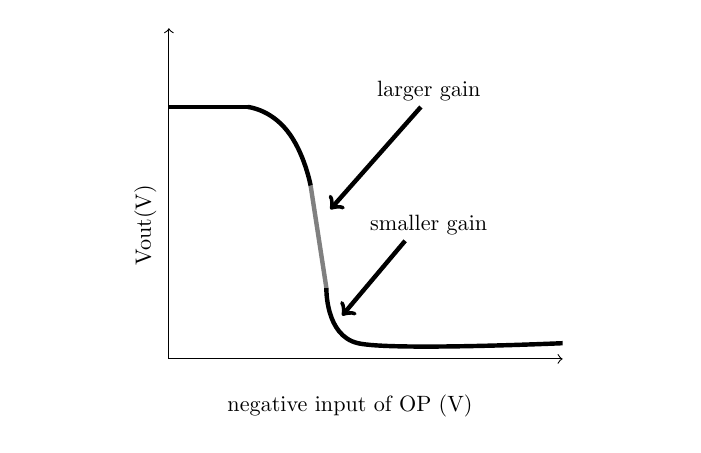
\begin{tikzpicture}
        \draw [black, ultra thick] plot coordinates { (0,4) (1,4) };
        \draw [black, ultra thick] plot [smooth, tension=1] coordinates { (1,4) (1.5,3.7) (1.8,3) };
        \draw [gray, ultra thick] plot [smooth, tension=1] coordinates { (1.8,3) (2,1.7) };
        \draw [black, ultra thick] plot [smooth, tension=0.5] coordinates { (2,1.7) (2.4,1) (5, 1) };

        \draw[->] (0, 0.8) -- (0, 5);
        \draw[->] (0, 0.8) -- (5, 0.8);
        \draw[->, ultra thick] (3.2, 4) -- (2.05,2.7);
        \draw[->, ultra thick] (3, 2.3) -- (2.2,1.35);
        \node[text width=5cm, scale=0.8, align=center] at (3.3, 2.5)
            {smaller gain};
        \node[text width=5cm, scale=0.8, align=center] at (3.3, 4.2)
            {larger gain};
        \node[text width=10cm, scale=0.8, align=center] at (2.3, 0.2)
            {negative input of OP (V)};
        \node[text width=5cm, scale=0.8, align=center, rotate=90] at (-0.3, 2.5)
            {Vout(V)};
    \end{tikzpicture}
    \caption{...}
    \label{fig:chip:line}
\end{figure}


\subsubsection*{Input Offset Voltage}
Another reason may be responsible for the low-current defect is the offset voltage at the input of the OP.

We examined the output voltage of TIA ($V_{TIA}$) of the Fig.\ref{fig:chip:IdIbiasVG} DC-sweep experiment.
It is shown in Fig.\ref{fig:chip:VTIA}.
Ideally, when feedback mechanism works well, $V_{TIA}$ should be equal to $V_{Ref}$(Fig.\ref{fig:chip:DCmode}).
However, the value of $V_{Ref}$ is $0.802 V$, which is smaller than $V_{TIA}$.
(This $V_{Ref}$ is connected to a constant voltage point inside the chip.
We know its value indirectly by measuring the drain voltage of nanowire since the drain of nanowire is kept to be same as $V_{Ref}$ by TIA.)
When the circuit works well, $V_{TIA}$ and $V_{Ref}$ is still different by $15m V$.
This voltage difference can result in an $150n A$ offset current flowing through TIA and into the nanowire device.
This offset current becomes remarkable when the $I_{bias}$ is less than $1\mu A$.

We suggest the reason that $V_{TIA}$ is large than $V_{Ref}$ is due to the offset voltage appearing at the input of the OP.
This speculation is reasonable through with respect to the layout, which will be discussed in the next section.

\begin{figure}[tbh!p]
    \centering
        \includegraphics[width=0.7\textwidth] {images/chapter6/gvt_0101Manual_VopiProblem.png}
    \caption{The $V_{TIA}$. The x-axis is the corresponding gate voltage.
                With the information from Fig.\ref{fig:chip:IdIbiasVG}, we found that the $V_{TIA}$ is not equal to $V_{Ref}$ no matter feedback mechanism works well or not.}
    \label{fig:chip:VTIA}
\end{figure}

Overall, the insufficient gain and the input offset may be the main reasons of the low-current defect.
Both of them relate to the OP block.
We then discuss these two reasons from the perspective of layout.

\subsection{The Design and Layout Problems of OP}
In the last section, me mentioned that the gain of OP is lower than we expected and there may exist an input offset voltage.
In this section, we will deduce that several layout and design flaws may be responsible for these two problems.

\begin{figure}[tbh!p]
    \centering
    \includegraphics[width=1\textwidth] {images/chapter6/OP_schematic.png}
    \caption{The left section is the schematics of the OP. The right section is a global circuit for generating the two global biasing voltage: $V_{bi}$, $V_{Ref}$.
                The Iin is an external current source.}
    \label{fig:chip:OPScem}
\end{figure}

\subsubsection{The Possible Reasons for Insufficient Gain}
The schematic presented in Fig.\ref{fig:chip:OPScem} contains two sections.
The left section is the body of the OP, while the right one is a global biasing circuit.




\section{Transient Measurement Mode}

\section{Dealing with the Device Variability Problem}

